%% LyX 2.1.1 created this file.  For more info, see http://www.lyx.org/.
%% Do not edit unless you really know what you are doing.
\documentclass[twocolumn,pre, reprint, nofootinbib]{revtex4-1}
\usepackage[latin9]{inputenc}
\setcounter{secnumdepth}{3}
\usepackage{amssymb}
\usepackage{graphicx}
\usepackage{amsmath}


\newcommand\blfootnote[1]{%
  \begingroup
  \renewcommand\thefootnote{}\footnote{#1}%
  \addtocounter{footnote}{-1}%
  \endgroup
}
\makeatletter

%%%%%%%%%%%%%%%%%%%%%%%%%%%%%% LyX specific LaTeX commands.
%% Because html converters don't know tabularnewline
\providecommand{\tabularnewline}{\\}

%%%%%%%%%%%%%%%%%%%%%%%%%%%%%% Textclass specific LaTeX commands.
% Fix a couple of bugs in REVTeX 4.1
\def\lovname{List of Videos}
\@ifundefined{textcolor}{}
{
 \definecolor{BLACK}{gray}{0}
 \definecolor{WHITE}{gray}{1}
 \definecolor{RED}{rgb}{1,0,0}
 \definecolor{GREEN}{rgb}{0,1,0}
 \definecolor{BLUE}{rgb}{0,0,1}
 \definecolor{CYAN}{cmyk}{1,0,0,0}
 \definecolor{MAGENTA}{cmyk}{0,1,0,0}
 \definecolor{YELLOW}{cmyk}{0,0,1,0}
}

\makeatother

\begin{document}

\title{Anti-ferromagnetic Ising Model in Hierarchical Networks }


\author{Xiang Cheng and Stefan Boettcher}

\affiliation{Department of Physics, Emory University, Atlanta, GA 30322, USA}
\begin{abstract}
The Ising antiferromagnet  is a convenient model of glassy dynamics.  It can introduce geometric frustrations and may give rise to a spin glass phase and glassy relaxation at low temperatures.  We apply the antiferromagnetic Ising model to 3 hierarchical networks which share features of both small world networks and regular lattices. Their recursive and fixed structures make them suitable for exact renormalization group analysis as well as numerical simulations. We first explore the dynamical behaviors using simulated annealing and discover an extremely slow relaxation at low temperatures. Then we employ the Wang-Landau algorithm to investigate the energy landscape and the corresponding equilibrium behaviors for different system sizes. Besides the Monte Carlo methods, renormalization group is used to study the equilibrium properties in the thermodynamic limit and to compare with the results from simulated annealing and Wang-Landau sampling. 
\smallskip 
\end{abstract}

\maketitle

\section{Introduction}

\label{sec:intro} 
BLANK

\section{RG Calculations}
\label{sec:RG}
 The setup of renormalization is started by separating the anti-ferromagnetic(AFM) Ising Hamiltonian into hierarchies
\begin{equation}
-\beta\mathcal{H} = \sum_{n=1}^{k-2} (-\beta \mathcal{H}_n)+ \mathcal{R}(K_2, K_3, \cdots)
\end{equation}
where $\mathcal{R}$ is the coupling beyond $\mathcal{H}_n$ of levels $k>2$. $\mathcal{H}_n$ depends on the interactions $K_0$ on the backbone and $L_0$, $L_1$, $K_1, \cdots$ among the long range couplings. We describe the RG procedure network by network. 


\subsection{RG Analysis of HNNP and HN6 without magnetic field}
\label{sec:HPRG}

\subsubsection{RG setup and procedures}
For HNNP and HN6, the $\mathcal{H}_n$ for each hierarchy is 
\begin{eqnarray}
\label{eq:hpz0}
 -\beta \mathcal{H}_n &=& K_0 \left(x_{n-2}x_{n-1} + x_{n-1}x_{n} +  x_{n}x_{n+1} +  x_{n+1}x_{n+2}\right) \nonumber \\ 
   && + K_1(x_{n-2}x_{n+1} + x_{n-1}x_{n+2}) + yL_1(x_{n-2} x_{n+2}) \nonumber \\
   && +L_0(x_{n-2}x_{n} + x_{n}x_{n+2})  + 4I 
\end{eqnarray}
I is a constant parameter emerging after the first step of RG, and its initial value is 0. $L_0$ also stands for the coupling term emerged in the RG process, and its initial value is also 0. All the initials values for these activity parameters are
\begin{equation}
\begin{array}{l}
\displaystyle I = 0 \\
\displaystyle K_0 < 0 \\
\displaystyle K_1 < 0 \\
\displaystyle L_0 = 0 \\
%\displaystyle L_1 < 0 \\
\end{array} 
\label{eq:init1}
\end{equation}
where $K_1$ is not changing in the RG flow because it is introduced `freshly' at every RG step. Therefore, it can be used as a reference of temperature. High temperatures $T \rightarrow \infty$ stands for $K_1\rightarrow -0$; while low temperatures $T\rightarrow 0$ corresponds to large $K_1 \rightarrow -\infty$.

The renormalization trace the sites $x_n$ and $x_{n+1}$ to get the renormalized form
\begin{equation}
\label{eq:hpz1}
 -\beta \mathcal{H}_n = 2I' +  K'_0 \left(x_{n-2}x_{n} +  x_{n}x_{n+2}\right) + L'_0(x_{n-2}x_{n+2})
 \end{equation}
 which is the same as that in HN3 and HN5. 
 \begin{equation}
\begin{array}{l}
\displaystyle C = e^{-4I} = e^{-A[0]}  \\
\displaystyle \kappa = e^{-4K_0} = A[1] \\
\displaystyle \lambda = e^{-4L_0} = A[2] \\
\displaystyle \mu = e^{-2K_1} = e^{-2L_1}= A[3] 
\end{array} 
\label{eq:activities}
\end{equation}
where $A[i]$ are the variables used in Mathematica calculations. The corresponding initial values are
 \begin{equation}
\begin{array}{l}
\displaystyle C = 1, A[0]=0 \\
\displaystyle \kappa = A[1]=\mu^2 > 1\\
\displaystyle \lambda = A[2] = \mu^{2y}\\
\displaystyle \mu = A[3] > 1 \\
\end{array} 
\label{eq:init1}
\end{equation}
In the calculation, we only need to specify the temperature $\mu$, then other initial values are determined accordingly.
The relationship between $\mu$ and $T$ is,  
\begin{equation}
\begin{array}{l}
\displaystyle T\rightarrow 0 \ \Leftrightarrow \ \ K_1 \rightarrow -\infty  \ \Leftrightarrow \ \ \mu \rightarrow \infty   \ \Leftrightarrow  \ \ {1}/{\mu}\rightarrow0\\
\displaystyle T\rightarrow \infty  \ \Leftrightarrow  \ K_1 \rightarrow -0 \ \Leftrightarrow  \ \ \mu \rightarrow 1 \  \ \Leftrightarrow  \ \  {1}/{\mu}\rightarrow 1 \\
\end{array} 
\label{eq:Ts}
\end{equation}
Eqs. \ref{eq:hpz0} and \ref{eq:hpz1} yields the RG recursions
\begin{equation}
\begin{array}{l}
\displaystyle \kappa' = \frac{\kappa \lambda (1+\mu)^2 }{(1+\mu\kappa)^2} \\
\\
\displaystyle \lambda' =\mu^{2y} \frac{(\kappa + \mu)^2} {(1 + \mu \kappa)^2} \\ \\
\displaystyle C' =  \frac{C^2 \kappa\mu^2} {(1+\mu^2) (\kappa+\mu) (1+ \mu\kappa)}   \\
\end{array} 
\label{eq:hpsol1}
\end{equation}
These solutions are also the same as those in Ref. \cite{boettcher2011rg}; we also reproduced the phase diagram of HNNP Ferromagnetic model
\begin{figure}
\centering 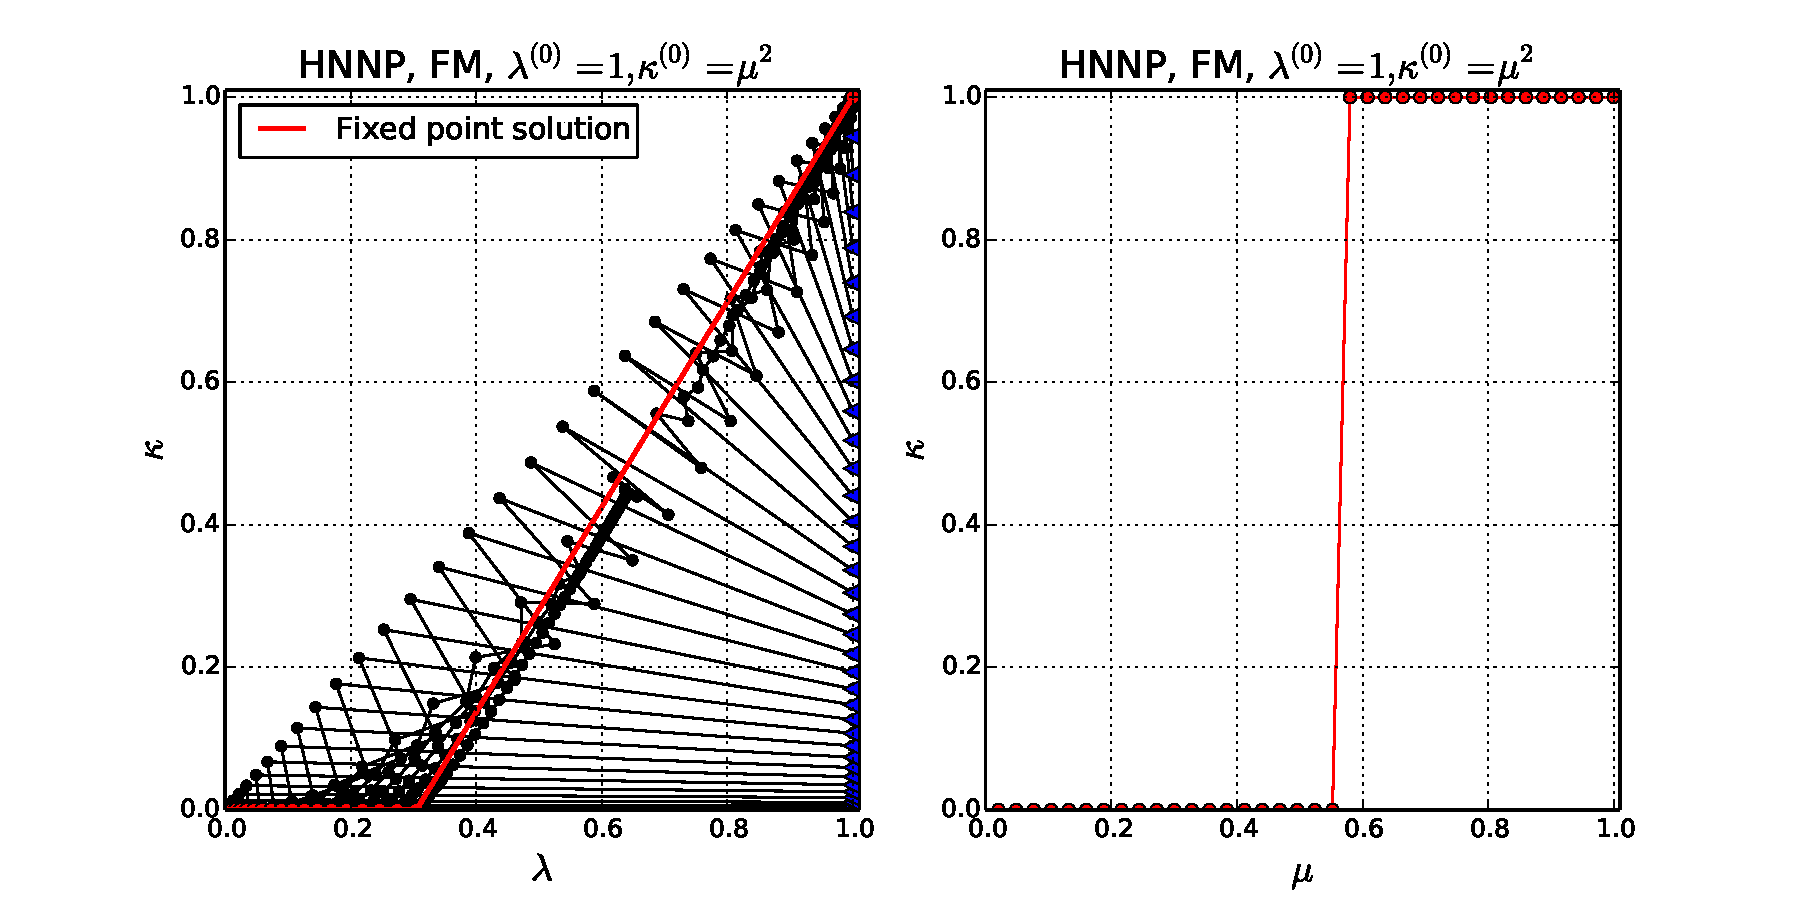
\includegraphics[width=1.05\columnwidth]{FM_HNNP_diagram.pdf}
\protect\caption{The Phase diagram of the Ising ferromagnet on HNNP. This figure is a reproduction of Fig. 10 in Ref. \cite{boettcher2011rg} to check the accuracy of the recursion solutions. The blue triangles are the initial values, and the red points are the fixed points after 500 RG steps.}
\label{fig:hpfm_dg} 
\end{figure}

\subsubsection{Fixed point analysis}
In the AFM scenario, for HNNP ($y = 0$), there are only 2 possible fixed points 
\begin{equation}
\begin{array}{l}
\kappa^* = 0, \ \lambda^* = \mu^2  \\ \\
\kappa^* = \lambda^* = 1 
\end{array}
\end{equation} 
{\it For HNNP, the actual fixed point is 1 for $\mu \le 3$ and `oscillating fixed points'  for $\mu > 3$}\\
--------------- Tranformation from $K$ to $J$ -----------------\\
For convenience, we set the the interaction constant $J=-1$ and Boltzmann constant $k_B=1$.
Then the variables of interest become
\begin{equation}
\begin{array}{l}
J^{(0)} = -1,  \\ \\
T = 2/\log(\mu) \\ \\
J^{(n)} = -\frac{T}{4}\log\kappa^{(n)}\\
\end{array}
\end{equation} 
---------------- Transformation Done --------------------\\
--------------- Fixed Point Stability -----------------\\
The Jocobian matrix
\begin{equation}
J_{11} = \frac{\partial \kappa'(\kappa, \lambda)}{\partial \kappa}=\frac{\lambda  (\mu +1)^2}{(\kappa  \mu +1)^2}-\frac{2 \kappa  \lambda  \mu  (\mu +1)^2}{(\kappa  \mu +1)^3}
\end{equation}

\begin{equation}
J_{12} = \frac{\partial \kappa'(\kappa, \lambda)}{\partial \lambda}=\frac{\kappa  (\mu +1)^2}{(\kappa  \mu +1)^2}
\end{equation}
\begin{equation}
J_{21} = \frac{\partial \lambda'(\kappa)}{\partial \kappa}=\frac{2 (\kappa +\mu ) \mu ^{2 y}}{(\kappa  \mu +1)^2}-\frac{2 (\kappa +\mu )^2 \mu ^{2 y+1}}{(\kappa  \mu +1)^3}
\end{equation}

\begin{equation}
J_{22} = \frac{\partial \lambda'(\kappa)}{\partial \lambda}=0
\end{equation}
--------------- Fixed Point Stability Done-----------------\\
In this AFM model, the fixed point analysis may be messy. Some figures may be not easy to make sense. In order to address the `messy' fixed point analysis, we show the analysis from 3 perspectives
\begin{enumerate}
\item Consistency \\
At low temperatures for certain values of $y$, $\kappa$ is oscillating with a certain pattern along the RG steps. The questions is whether the oscillation pattern is changing for different number of RG steps. Our analysis shows that the pattern does not change after $\sim 1000$ RG steps. In other words, for example, the oscillation pattern of of steps $(1000 \sim 5000)$ is the same as that  of steps $(5000 \sim 9000)$, $(9000 \sim 14000)$, etc. Fig. \ref{fig:hp6_cons} is an example of this `consistency analysis'. Note for different $y$ and $\mu$, the histogram curves may be very different. It is easy to see the `disorderness' of the fixed points in the following two perspectives. 

\item Histogram of $\kappa$ at different $\mu$ and $y$
Generally, at high temperatures ($\mu$ is small), there is usually one stable fixed point; but, at low temperatures ($\mu$ is big), $\kappa$ is usually oscillating. The lower the temperature is, the wider $\kappa$ spreads. Fig. \ref{fig:hp6_hist_p} (positive $y$) and Fig. \ref{fig:hp6_hist_n} (negative $y$) show the distribution of different $\kappa$. The next figures (Figs. \ref{fig:hp6_kmu_p} and \ref{fig:hp6_kmu_n}) can help explain.

\item All values of $\kappa$ at different $\mu$ and $y$. Inspired by Ref. \cite{mckay1982} Fig 2, we plot all the $\kappa$ in the RG steps (steps $18000 \sim 20000$). Each ($\kappa, 1/\mu$) is a data point in Figs. \ref{fig:hp6_kmu_p} and \ref{fig:hp6_kmu_n}. You can see why the histogram plots are messy. The values of $\kappa$ covers a large range and may be not very discrete. 
\end{enumerate}
When $y<2.0$, the whole system became similar to ferromagnetic model as shown in Fig. \ref{fig:hp6_kmu_n2}. 

More future work is needed to explain the chaotic bands and the transition to chaotic bands.

\begin{figure}
\centering 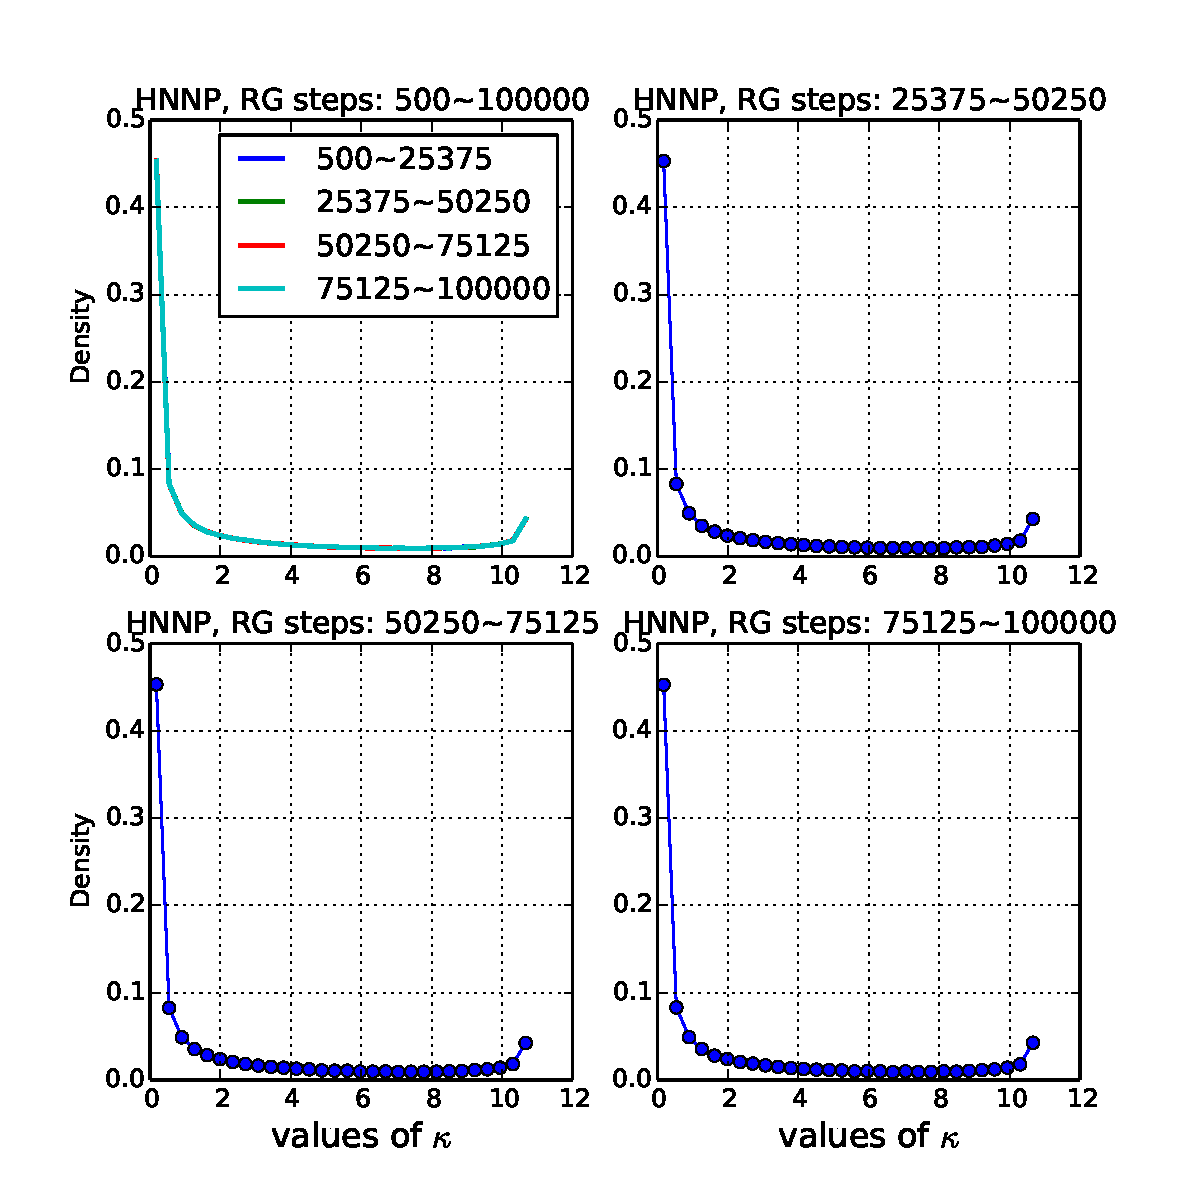
\includegraphics[width=1.0\columnwidth]{HNNP_cons.pdf}
\protect\caption{Consistency of the pattern for different RG steps ($y=0; \mu = 4$). The first figure is the histogram of all the RG steps; while the rest three figures are for different step-range. They are the same, which is important for further analysis. }
\label{fig:hp6_cons} 
\end{figure}

\begin{figure*}
\centering 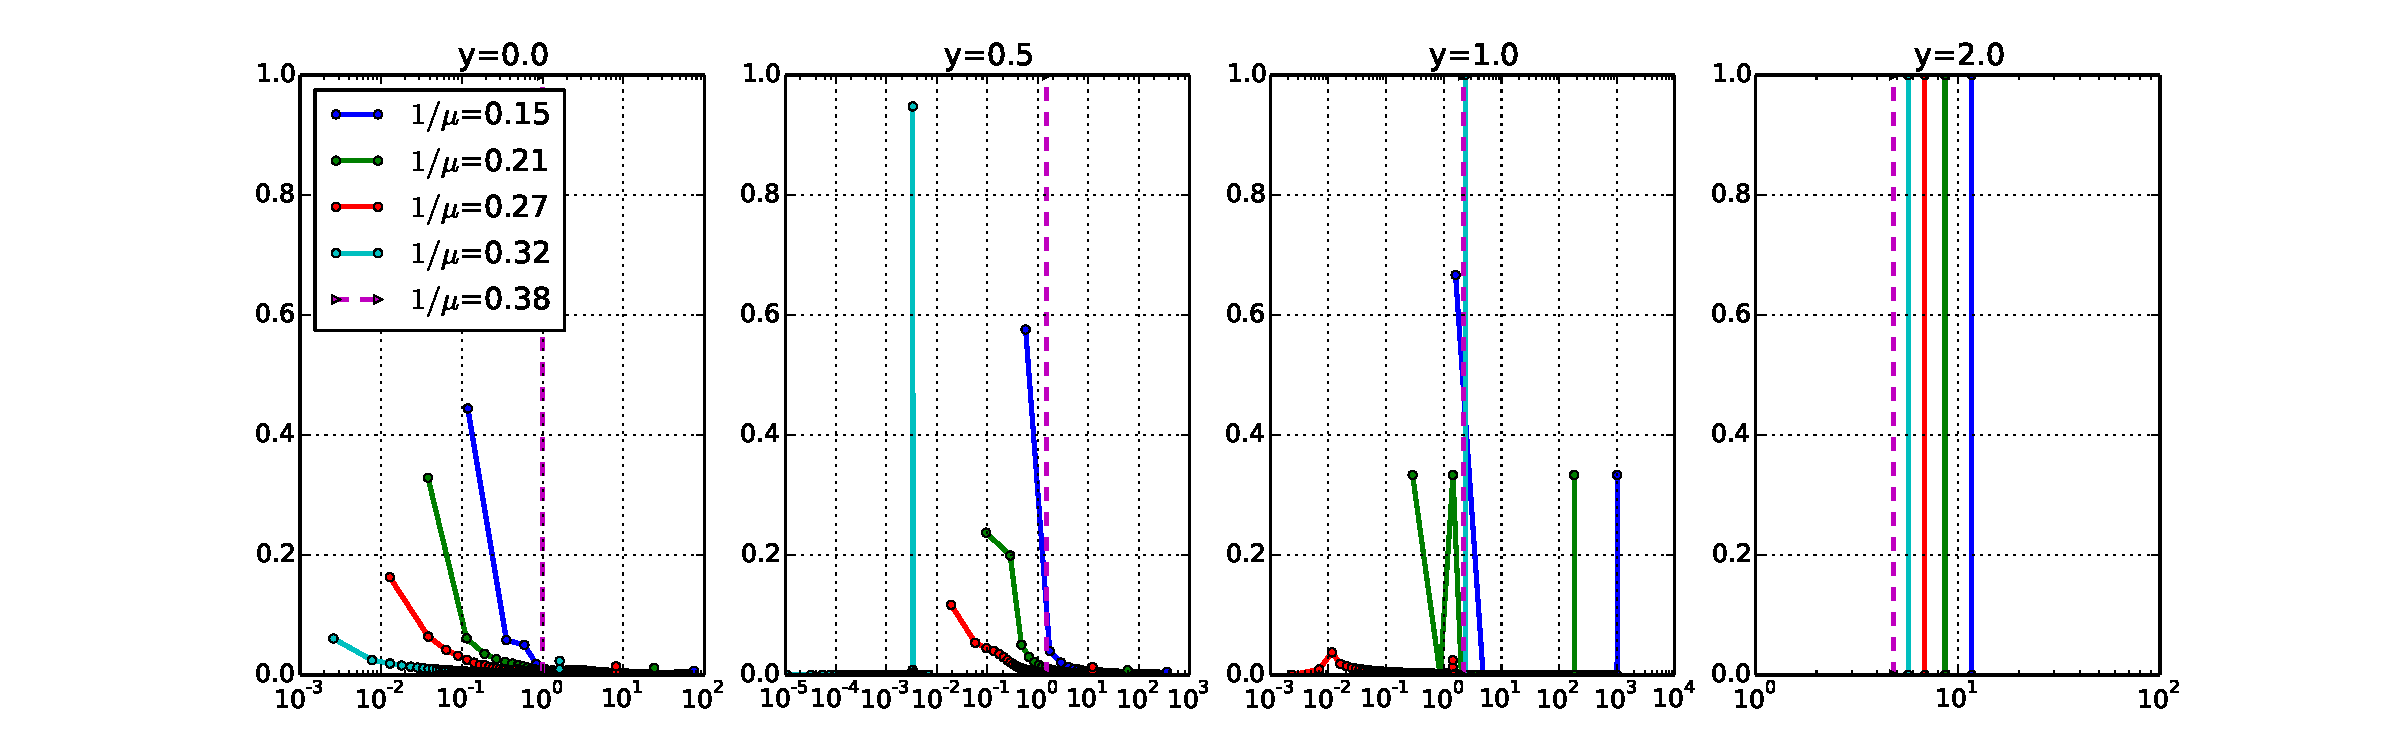
\includegraphics[width=2.0\columnwidth]{HP6_FP_freq_ys_p.pdf}
\protect\caption{Histogram of $\kappa$ at different $\mu$ and positive $y$ of steps $1000 \sim 20000$ (Density vs $\kappa$). For y = 0 (HNNP), the transition happens at $\mu=3$, i.e., for $\mu \le 3.0$, there is one fixed point at $\kappa = 1$, while, for $\mu>3.0$, $\kappa$ is oscillating and never converge to one point. Figs. \ref{fig:hp6_kmu_p} and \ref{fig:hp6_kmu_n} can help explain.}
\label{fig:hp6_hist_p} 
\end{figure*}

\begin{figure*}
\centering 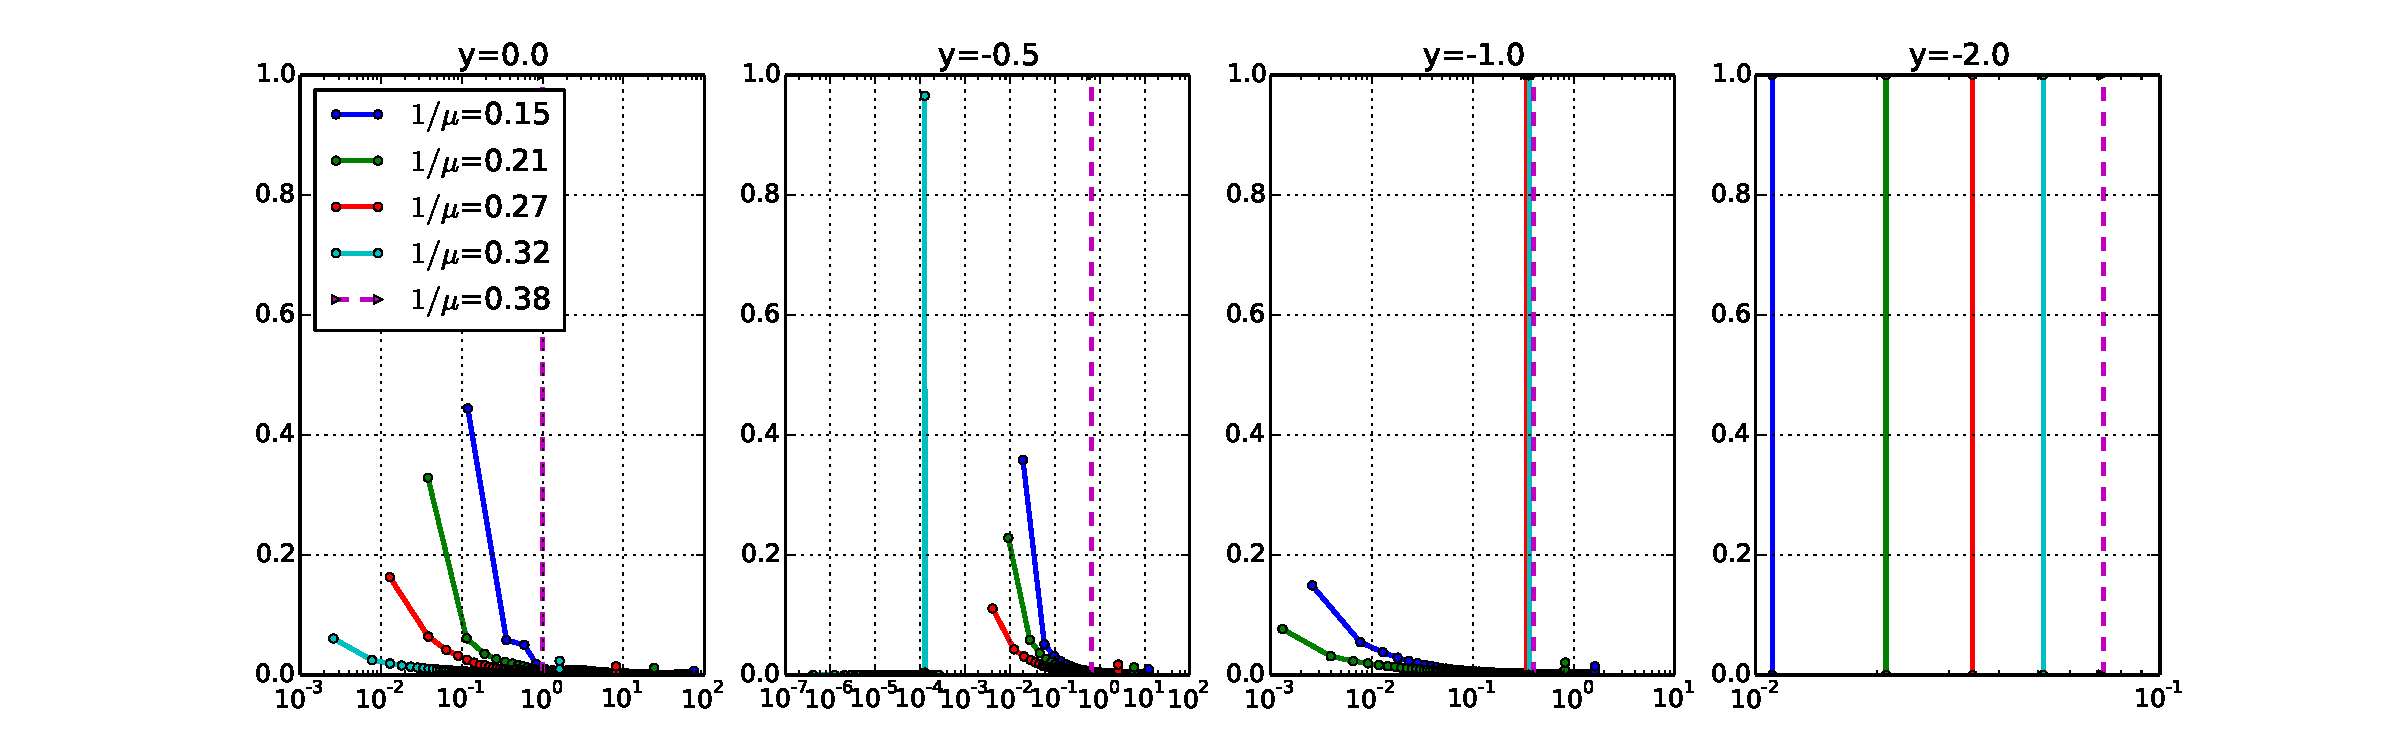
\includegraphics[width=2.0\columnwidth]{HP6_FP_freq_ys_n.pdf}
\protect\caption{Histogram of $\kappa$ at different $\mu$ and negative $y$ of steps $1000 \sim 20000$ (Density vs $\kappa$). The legend in the 1st  subfigure works for all subfigures.  Figs. \ref{fig:hp6_kmu_p} and \ref{fig:hp6_kmu_n} can help explain.}
\label{fig:hp6_hist_n} 
\end{figure*}


\begin{figure}
\centering 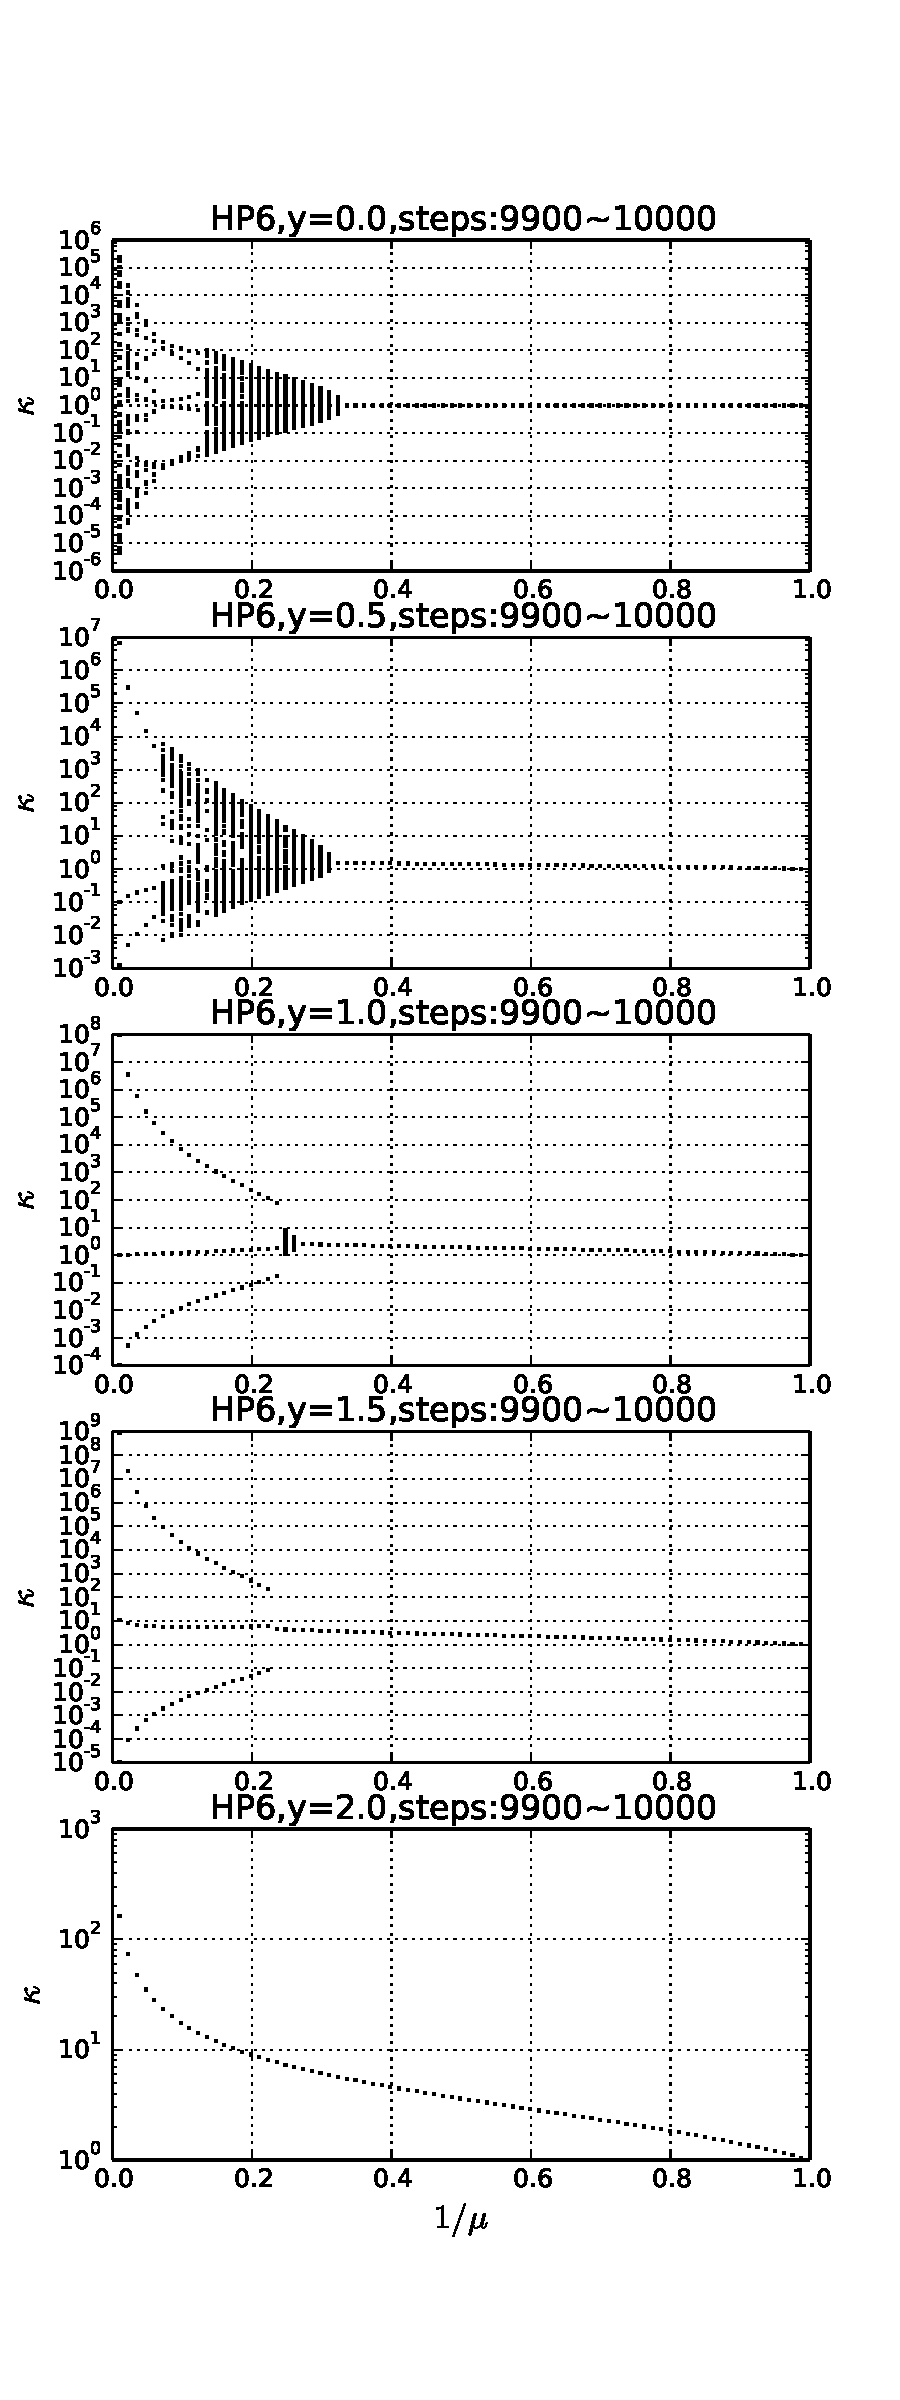
\includegraphics[width=1.0\columnwidth]{HP6_AFM_k_mu_N10000l100ys_np.pdf}
\protect\caption{All values of $\kappa$ with position $y$ for steps $18000 ~ 20000$. This figure is similar to Ref \cite{mckay1982} Fig.2. The reason of just using 2000 (20000 - 18000) is because of cercern of figure file size. The more steps included, the more data points in the figure, which makes the figure file very large and slow to open.}
\label{fig:hp6_kmu_p} 
\end{figure}

\begin{figure}
\centering 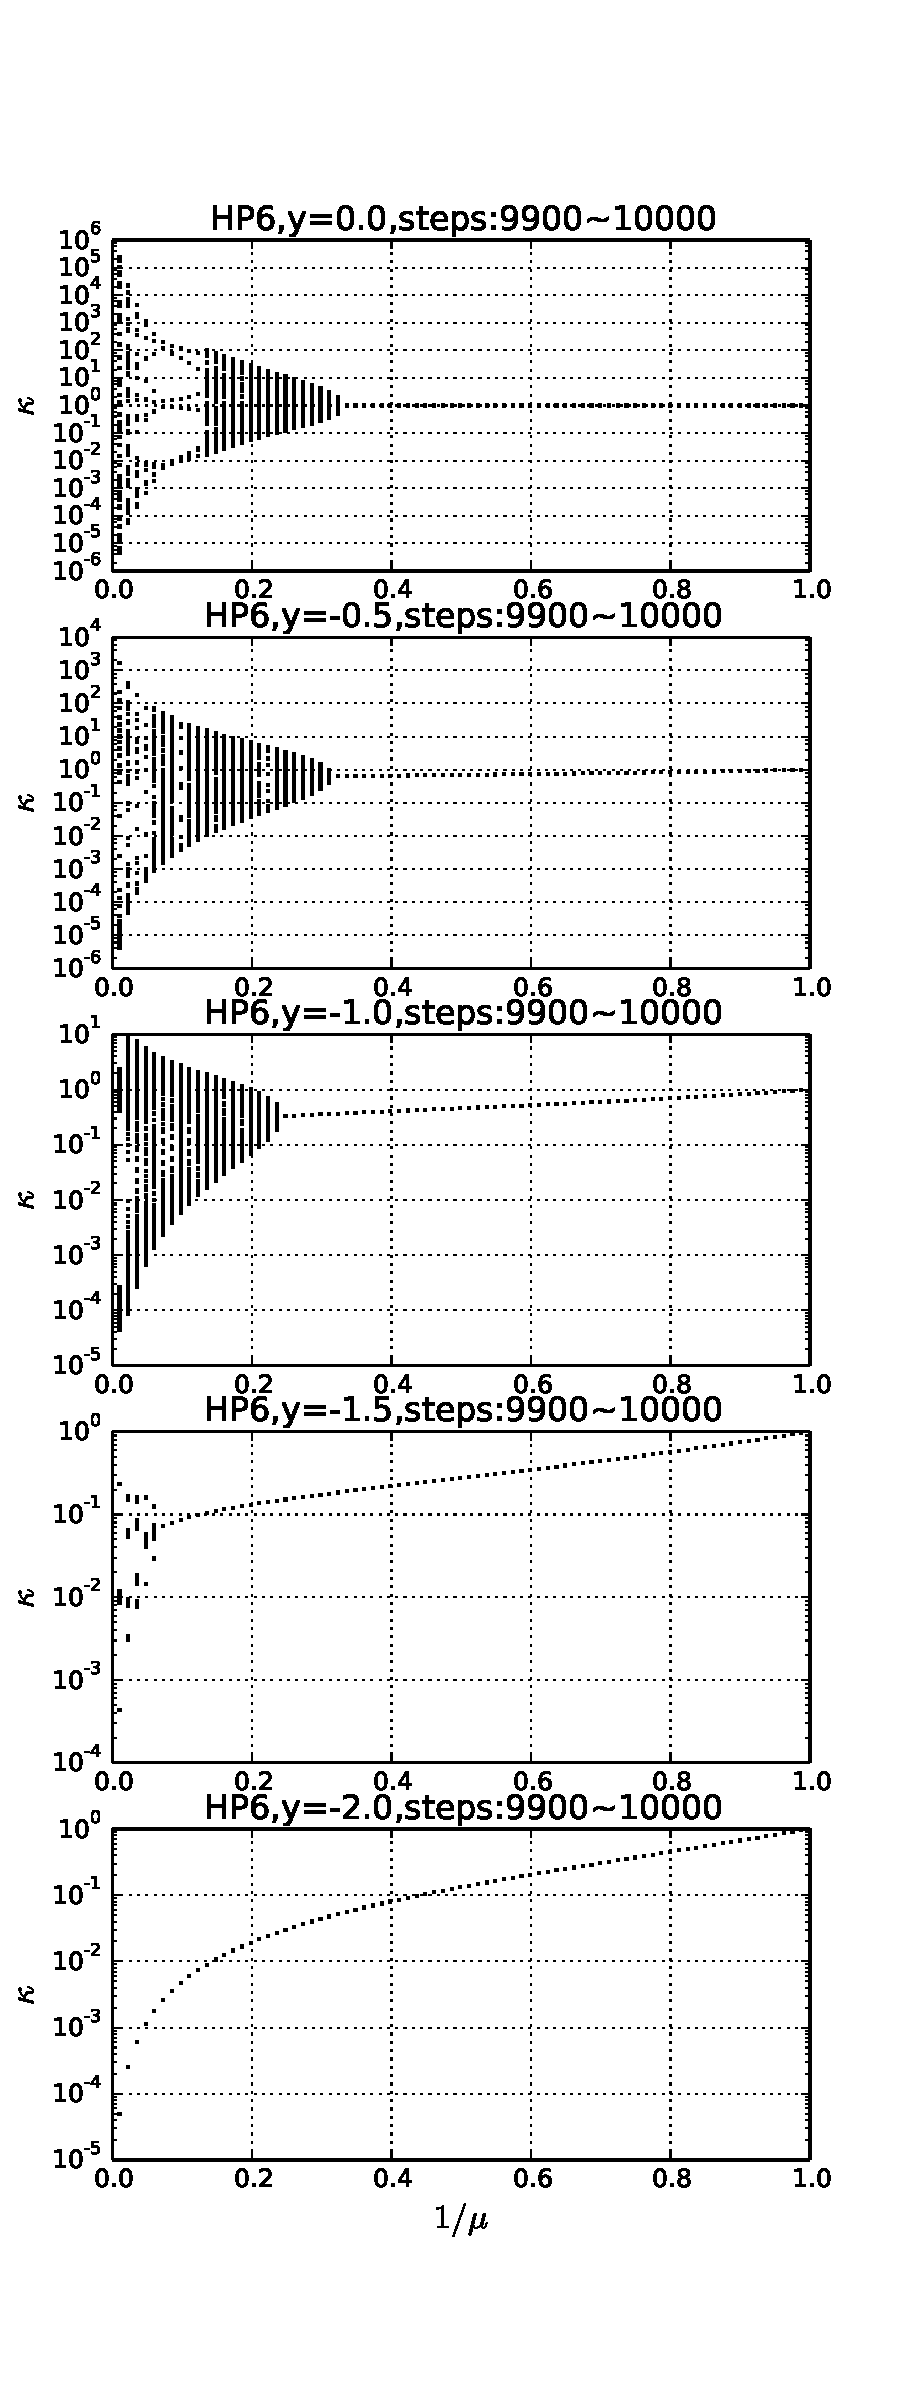
\includegraphics[width=1.0\columnwidth]{HP6_AFM_k_mu_N10000l100ys_nn.pdf}
\protect\caption{All values of $\kappa$  with negative $y$ for steps $18000 ~ 20000$. This figure is similar to Ref \cite{mckay1982} Fig.2. }
\label{fig:hp6_kmu_n} 
\end{figure}


\begin{figure}
\centering 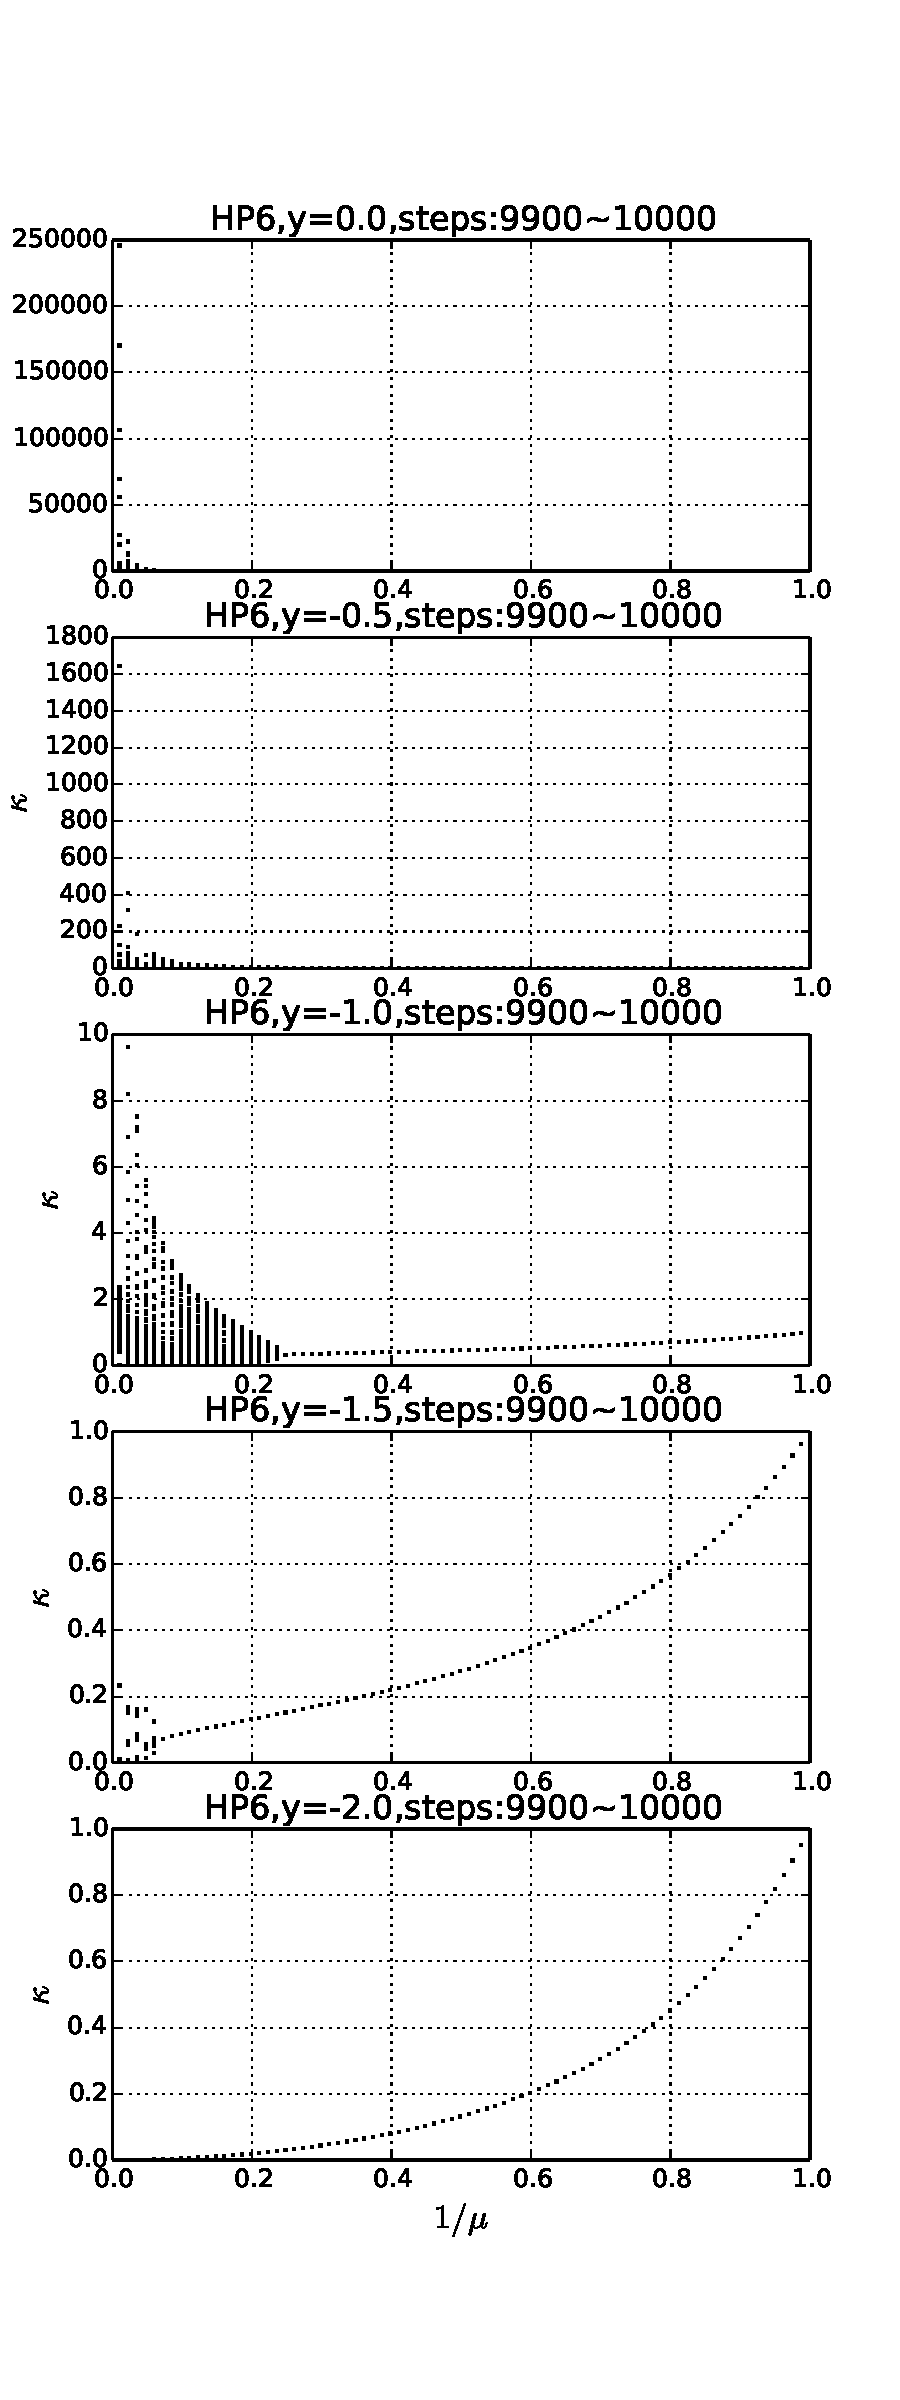
\includegraphics[width=1.0\columnwidth]{HP6_AFM_k_mu_n_normal.pdf}
\protect\caption{All values of $\kappa$  with negative $y$ for steps $18000 ~ 20000$. This figure is similar to Ref \cite{mckay1982} Fig.2. }
\label{fig:hp6_kmu_n2} 
\end{figure}




\subsection{RG Analysis of HN3 and HN5 without magnetic field}
\label{sec:HN35RG}

\subsubsection{RG setup and procedures}
For HN3 and HN5, the $\mathcal{H}_n$ for each hierarchy is
\begin{eqnarray}
\label{eq:z0}
 -\beta \mathcal{H}_n &=& K_0 \left(x_{n-2}x_{n-1} + x_{n-1}x_{n} +  x_{n}x_{n+1} +  x_{n+1}x_{n+2}\right) \nonumber \\ 
   && + K_1(x_{n-1}x_{n+1}) + L_0(x_{n-2}x_{n} + x_{n}x_{n+2}) \nonumber \\
   && + y L_1 (x_{n-2} x_{n+2})  + 4I 
\end{eqnarray}
where $y$ is 0 for HN3 and 1 for HN5. $I$ is a constant emerging since the first step of RG, and its initial value is 0. $L_0$ also stands for the coupling term emerged in the RG flow, and its initial value is also 0. The \underline{\emph{initial values}} for these parameters are
\begin{equation}
\begin{array}{l}
\displaystyle I = 0 \\
\displaystyle K_0 < 0 \\
\displaystyle K_1 < 0 \\
\displaystyle L_0 = 0 \\
\displaystyle L_1 < 0 \\
\end{array} 
\label{eq:init1}
\end{equation}
where $K_1$ is not changing in the RG flow because it is introduced again at every RG step. Therefore, it can be used as a reference of temperature. High temperatures $T \rightarrow \infty$ stands for $K_1\rightarrow -0$; while low temperatures $T\rightarrow 0$ corresponds to large $K_1 \rightarrow -\infty$.

After tracing the sites $x_{n-1}$ and $x_{n+1}$, in order to use RG, we have to get this form of equation
\begin{equation}
\label{eq:z1}
 -\beta \mathcal{H}_n = 2I' +  K'_0 \left(x_{n-2}x_{n} +  x_{n}x_{n+2}\right) + L'_0(x_{n-2}x_{n+2})
 \end{equation}
 which is `half' of original RG setup.
For convenience of the partition function and Mathematica calculation, we rewrite these parameters as
\begin{equation}
\begin{array}{l}
\displaystyle C = e^{-4I} = e^{-A[0]}  \\
\displaystyle \kappa = e^{-4K_0} = A[1] \\
\displaystyle \lambda = e^{-4L_0} = A[2] \\
\displaystyle \mu = e^{-2K_1} = e^{-2L_1} = A[3] 
\end{array} 
\label{eq:activities}
\end{equation}
The array $\{A[i]\}$ is used in the Mathematica calculations. The pre-factors of $K_0, K_1, I, {\rm and} L_1$ is for the convenience of the RG calculations. The reason to use exponential form for $C$ and $A[0]$ is to utilize more precision in Mathematica. Thus, the  \underline{\emph{initial values}}  for them are
\begin{equation}
\begin{array}{l}
\displaystyle C = 1, A[0]=0 \\
\displaystyle \kappa = A[1] = \mu^2 > 1\\
\displaystyle \lambda = A[2] =\mu^{2y} = 1\\
\displaystyle \mu = A[3] >1 \\
\end{array} 
\label{eq:init1}
\end{equation}
Generally, we only specify $\mu$ in the first step of RG; the initial values for HN3($y=0$) and HN5($y=1$) are determined by $\mu$ and $y$.

The relationship between $\mu$ and $T$ is the opposite as between temperature $T$  and $K_1$,  
\begin{equation}
\begin{array}{l}
\displaystyle T\rightarrow 0 \ \Leftrightarrow \ \ K_1 \rightarrow -\infty  \ \Leftrightarrow \ \ \mu \rightarrow \infty   \ \Leftrightarrow  \ \ {1}/{\mu}\rightarrow0\\
\displaystyle T\rightarrow \infty  \ \Leftrightarrow  \ K_1 \rightarrow -0 \ \Leftrightarrow  \ \ \mu \rightarrow 1 \  \ \Leftrightarrow  \ \  {1}/{\mu}\rightarrow 1 \\
\end{array} 
\label{eq:Ts}
\end{equation}
By tracing over all the $\{x_n\}$ in Eq. \ref{eq:z0} and Eq. \ref{eq:z1}, we can get equations and the following solutions
\begin{equation}
\begin{array}{l}
\displaystyle \kappa' = \frac{2\kappa \lambda (1+\mu) }{\kappa^2+2\mu \kappa +1} \\
\\
\displaystyle \lambda' = \mu^{2y} \frac{(1+\mu)(1+\kappa)^2}{2(\kappa^2+2\mu \kappa +1)}\\ \\
\displaystyle C' =  \frac{C^2 \kappa\mu}{\sqrt{2} (1+\kappa) (1+\mu)^{3/2}  \sqrt{ \kappa^2+2\mu \kappa +1}}   \\
\end{array} 
\label{eq:sol1}
\end{equation}

In Mathematica, what we get equivalently is actually
\begin{equation}
\begin{array}{l}

\displaystyle A'[1] = \frac{2A[1] A[2] (1+\mu) }{1+2\mu A[1] +A[1]^2} \\
\\
\displaystyle A'[2] = \mu^{2y}\frac{(1+\mu)(1+A[1])^2}{2(1+2\mu A[1]+A[1])}\\ \\ 
\displaystyle A'[0] =  \frac{1}{2} \log \left( \frac{e^{-4A[0]} \mu^2 A[1]^2}{2(1+\mu)^3 (1+A[1])^2 (1+2\mu A[1]+A[1]^2)}  \right) 
\end{array} 
\label{eq:activities}
\end{equation}

\subsubsection{Fixed point analysis}
For HN3 with $y=0$, we get 2 analytical fixed point solutions which are
\begin{equation}
\begin{array}{l}
\displaystyle \kappa = 1, \lambda =1;  \\
\displaystyle \kappa = 0, \lambda =\frac{1+\mu}{2} 
\end{array} 
\label{eq:fps3}
\end{equation}
where only the first one is a stable fixed point solution. The second one is only stable at infinitely high temperatures; any finite temperatures lead to the fixed point $\kappa =1, \lambda = 1.$ \\

For HN5 with $y=1$, the fixed points are more interesting. The fixed point solution are
\begin{equation}
\kappa = 0, \ \  \lambda = \mu^{2y}\frac{\mu+1}{2}
\label{eq:fps5}
\end{equation}

\begin{equation}
\kappa = \frac{1}{2}\left[\mu^2 -\mu + \sqrt{(\mu+1)(\mu^3 - 3\mu^2 +8\mu-4)} \right]
\label{eq:fps51}
\end{equation}

\begin{equation}
\lambda = \frac{\mu}{4}\left[\mu^2 -\mu+2 + \sqrt{(\mu+1)(\mu^3 - 3\mu^2 +8\mu-4)} \right]
\label{eq:fps52}
\end{equation}
For the parameter of interest $\kappa$, its solution Eq.\ref{eq:fps51} can be written in a general form as a function of $\mu$ ($\mu>1$)
\begin{equation}
\kappa = \frac{1}{2}\left[\mu^{1+y}+\mu^{y} -2\mu + \sqrt{4\left( \mu^{1+y} + \mu^{y} - 1\right)+\left( \mu^{1+y} + \mu^{y} - 2\mu\right)^2} \right]
\label{eq:fps_k}
\end{equation}
$\kappa$ changes with $\mu$; the values of $\mu$ satisfying $\kappa(\mu)=0$ are likely to be the phase transition temperatures. After transformation of Eq.\ref{eq:fps_k}, the equation $\kappa(\mu)=0$ can be rewritten as 
\begin{equation}
\mu^{1+y} + \mu^y -1 =0
\end{equation}
where, for any values of $y$, the real roots of  $\mu>1$ are the acceptable solutions. The examples with specific values of $y$ is listed below
\begin{equation}
\begin{array}{l}
\displaystyle y \rightarrow \infty:\  \mu^{1+y} + \mu^y -1 =0; \ \mu \rightarrow 1 ({\rm\ FM,\  } T\rightarrow \infty) \\ \\ \\
\displaystyle y = 2:\  \mu^3 + \mu^2-1 =0; \ \mu =0.754878 {\rm\ ( FM)} \\ \\ \\
\displaystyle y = 1:\  \mu^2 + \mu -1 =0; \ \mu =\frac{\sqrt{5}-1}{2} {\rm\  (FM, HN5)} \\ \\ \\
\displaystyle y = \frac{\log(3/2)}{\log2}:\  \mu^{1+y} + \mu^y -1 =0; \ \mu =1/2 {\rm\  (FM)}\\ \\ \\
\displaystyle y = 0:\  \mu + \mu^0 -1 =0; \ \mu =0 \ ({\rm FM, HN3, \ }T=0) \\ \\ \\
\displaystyle y = -0.5:\  \sqrt{\mu} + \frac{1}{\sqrt{\mu}} -1 =0;  {\rm\  no\ real \ solution} \\ \\ \\
\displaystyle y = -1:\  \mu^0 + \frac{1}{\mu} -1 =0; \ \mu \rightarrow \infty \ ({\rm AFM, \ }T=0 )\\ \\ \\
\displaystyle y = -1.5:\  \frac{1}{\sqrt{\mu}} + \frac{1}{\sqrt{\mu^{3}}} -1 =0; \ \mu = 2.147899 {\rm \ (AFM)}\\ \\ \\
\displaystyle y = -2:\  \frac{1}{\mu} + \frac{1}{\mu^{2}} -1 =0; \ \mu = 1.618034 {\rm \ (AFM)}\\ \\ \\
\displaystyle y \rightarrow \infty:\   \mu^{1+y} + \mu^y -1 =0;\ \mu \rightarrow 1 \ ({\rm AFM, \ }T\rightarrow\infty)\\ \\ \\ \nonumber
\end{array} 
\label{eq:sol_y}
\end{equation}

\begin{figure*}
\centering 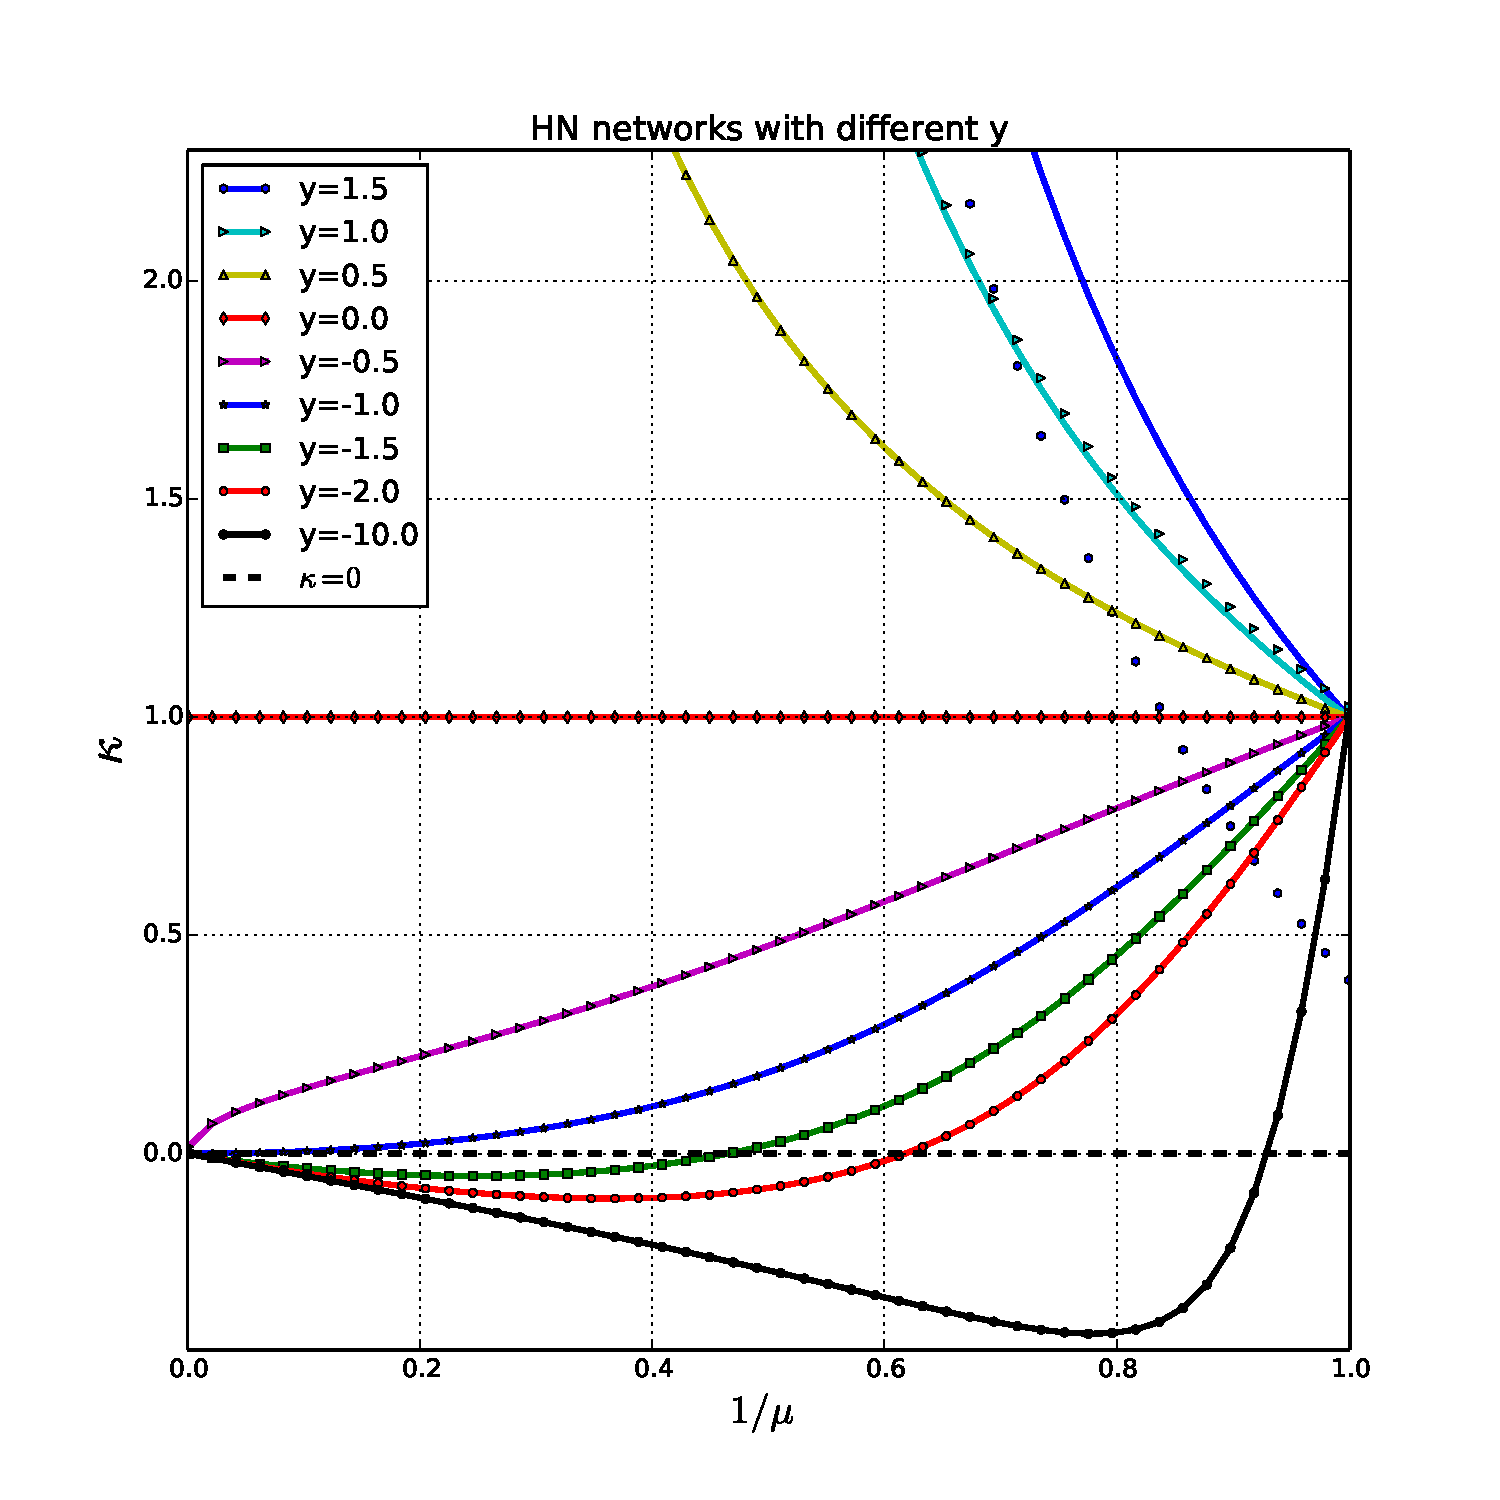
\includegraphics[width=2\columnwidth]{AFM_HN_ys_kvsmu.pdf}
\protect\caption{$\kappa$ vs $1/\mu$ calculating using Eq.\ref{eq:fps_k}. In AF model, our temperature parameter $\mu$ is greater than 1. In this case, $1/\mu = 0 \Leftrightarrow T = 0$; $1/\mu = 1 \Leftrightarrow T\rightarrow \infty $ }
\label{fig:HN35_ys} 
\end{figure*}

%\begin{figure*}
%\centering 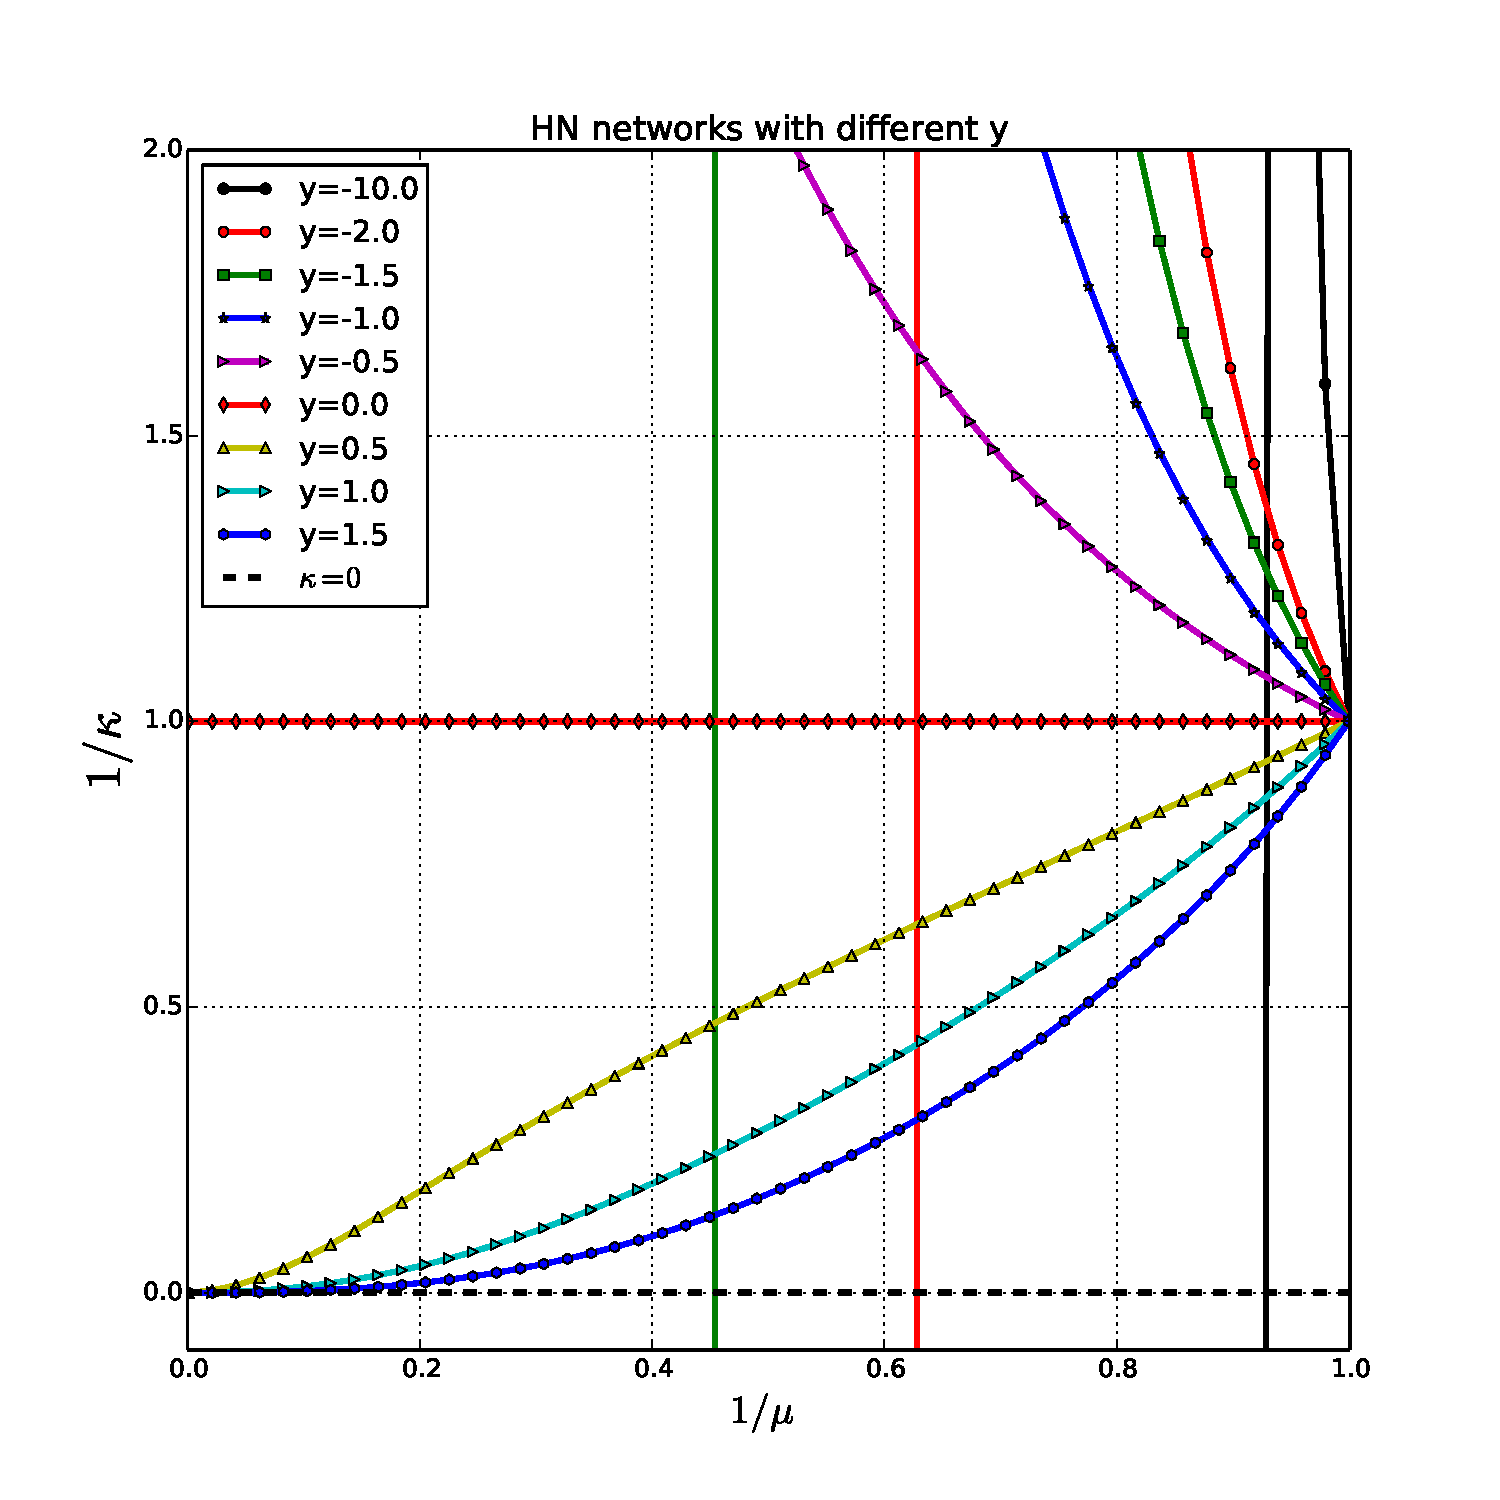
\includegraphics[width=2\columnwidth]{AFM_HN_ys_1okvsmu.pdf}
%\protect\caption{$1/\kappa$ vs $1/\mu$ calculating using Eq.\ref{eq:fps_k}. The black, red, and green vertical lines are from $y=-10, -2.0,\ {\rm and\ } -1.5$, respectively. They are due to the intersection of these curves and $\kappa = 0$. In AF model, $1/\mu = 0 \Leftrightarrow T = 0$; $1/\mu = 1 \Leftrightarrow T\rightarrow \infty $ }
%\label{fig:HN35_ys} 
%\end{figure*}
%\section*{Acknowledgements}
%We thank the U. S. National Science Foundation for its support through
%grant DMR-1207431.

\bibliographystyle{apsrev4-1}
%\bibliography{Jamming}
\bibliography{cheng}

\end{document}
